\section{Planning and reinforcement learning}\label{section:bg:planning-rl}

RL can present an extremely low efficiency when it is learning in bad conditions.
Without modifying the RL algorithm, it is possible to modify the environment in such a way as to facilitate learning
in a more straightforward context.
The solution to a reinforcement learning problem is a policy, denoted by $\pi$, that maximises the sum of expected rewards.
To ascertain the action that maximises the sum of expected rewards from a given state, an agent must explore all
possible actions in all possible states, as it is unable to evaluate each pair of states and actions otherwise.
It can thus be concluded that reducing the size of the environment in which the RL algorithm is operating will in fact
make it easier for it to learn.
The optimal action in a given space is contingent on the actions that are feasible.
Consequently, it is not possible to reduce the size of the research space over the action space.
However, a reduction in the research space through the investigation of a specific subset of the state space may result
in the elimination of numerous rewarding states.
Consequently, the optimal policy of the sub-problem may diverge from that of the initial problem.
In such cases, the creation of sub-tasks, each with its own reward function, becomes imperative.
The subsequent challenge is to ascertain the sequence in which these sub-tasks are to be executed.
This determination can be facilitated by an alternative policy, which will select the necessary sub-task.
This results in the existence of two distinct policies: a local policy, denoted by $\pi_l$, and a global policy, denoted by $\pi_g$.
The local policy will solve simple tasks chosen by the global policy, and the global policy will interact with a
simpler environment that is a composition of the local policy and the original environment.
This paradigm is represented in Figure~\ref{figure:bg:plan-rl:wrapped-agent}.

\begin{definition}[stochastic hierarchical policy]
    A stochastic policy $\pi(a|s)$ can be express in the context of hierarchical agents by:
    \begin{equation}
        \begin{split}
            \pi(a|s) &= \int_{A'}\pi_l(a \mid a', s')\pi_g(a' \mid s) da' \\
            &= \mathbb{E}_{a'\sim \pi_g(s)} \left [ \pi_l(a \mid a', s') \right ]
        \end{split}
    \end{equation}
    Where $a' \in A'$ is a global action, and $A'$ is the global actions space.
\end{definition}


\begin{figure}
    \centering
    \begin{tikzpicture}[scale=1, transform shape]
        \tikzstyle{every node}=[font=\sffamily\small]
        \useasboundingbox (0, 0) rectangle (10, 6);

        % Global agent
        \coordinate (G) at (0, 5);  % Global agent position
        \draw[orange, rounded corners=10pt, thick] (G) rectangle ($(G) + (4.5,-2)$);
        \node[anchor=north west, text width=\linewidth, color=orange] at ($(G) + (0.1,-0.1)$) {Global Agent};
        % Global policy
        \coordinate (Gp) at ($(G) + (2.5,-0.2)$);  % Global agent position
        \draw[orange, rounded corners=5pt, very thick, dashed] (Gp) rectangle ($(Gp) + (1.5,-1.5)$);
        \node[anchor=north west, text width=\linewidth, color=orange] at ($(Gp) + (0.1,-0.1)$) {Global \\ policy};

        % Control agent
        \coordinate (C) at (0, 2.5);  % Control agent position
        \draw[red, rounded corners=10pt, thick] (C) rectangle ($(C) + (4.5,-2)$);
        \node[anchor=north west, text width=\linewidth, color=red] at ($(C) + (0.1,-0.1)$) {Control Agent};
        % Control policy
        \coordinate (Cp) at ($(C) + (2.5,-0.2)$);  % Control agent position
        \draw[red, rounded corners=5pt, very thick, dashed] (Cp) rectangle ($(Cp) + (1.5,-1.5)$);
        \node[anchor=north west, text width=\linewidth, color=red] at ($(Cp) + (0.1,-0.1)$) {Control \\ policy};

        % Environment
        \coordinate (E) at (6,3.75);  % Control agent position
        \draw[green, rounded corners=10pt, thick] (E) rectangle ($(E) + (2.5, -2)$);
        \node[anchor=north west, text width=\linewidth, color=green] at ($(E) + (0.1, -0.1)$) {Environment};

        % ARROWS
        %> State
        \draw[->, line width=1.5pt, blue] ($(Gp) + (4.5,-0.5)$) -- ($(Gp) + (1.5,-0.5)$);
        \draw[->, line width=1.5pt, blue, rounded corners=5pt] ($(E) + (1.25, 0)$) --  ($(E|-Gp) + (1.25, -0.5)$) -- ($(Gp) + (2.5,-0.5)$) -- ($(Cp) + (2.5,-0.5)$) -- ($(Cp) + (1.5,-0.5)$);
        \node[anchor=north west, text width=\linewidth, color=blue] at (5.9,4.7) {$s$};

        %> Action
        \draw[->, line width=1.5pt, red, rounded corners=5pt] ($(Cp) + (1.5,-1)$) -- ($(E|-Cp) + (1.25, -1)$) -- ($(E) + (1.25, -2)$);
        \node[anchor=north west, text width=\linewidth, color=red] at (5.7,1.2) {$a$};

        %> Global action
        \draw[->, line width=1.5pt, orange] ($(Gp) + (0.75,-1.5)$) -- ($(Cp) + (0.75,0)$);
        \node[anchor=north west, text width=\linewidth, color=red] at ($(Gp) + (0.2, -1.8)$) {$a'$};

        % Steps markers
        \node[draw, circle, thick] at (4,3.6) {1};
        \node[draw, circle, thick] at (3.1,1) {2};

        % Legend
        \coordinate (L) at (8, 4.8);  % Control agent position
        \draw[->, line width=1.5pt, blue] (L) -- ($(L) + (0.7,0)$);
        \node[anchor=north west, text width=\linewidth, color=blue] at ($(L) + (0.8,0.25)$) {state};
        \draw[->, line width=1.5pt, red] ($(L) + (0,-0.4)$) -- ($(L) + (0.7,-0.4)$);
        \node[anchor=north west, text width=\linewidth, color=red] at ($(L) + (0.8,-0.15)$) {action};
        \draw[->, line width=1.5pt, orange] ($(L) + (0,-0.8)$) -- ($(L) + (0.7,-0.8)$);
        \node[anchor=north west, text width=\linewidth, color=orange] at ($(L) + (0.8,-0.55)$) {global action};
    \end{tikzpicture}
    \caption{Hierarchical agent diagram. At step 1, the state is given to the global policy to produce a global action
        (orange arrow) $a'$ that will be used to contition the control policy. At step 2, the control policy produce a
        control action $a$ using the state, and the global policy conditioning action.}
    \label{figure:bg:plan-rl:wrapped-agent}
\end{figure}

This definition underscores the fact that the stochastic local policy, denoted by $p_l$, is defined on
$S \times A \times A'$ and that the stochastic global policy, denoted by $\pi_g$, is defined on $S \times A'$.
From this perspective, it does not appear that the scope of our research has been reduced.
In practice, the control policy is required to solve sub-tasks, thereby facilitating the identification of rewarding
state-action pairs.
Despite the fact that the local policy is defined on the entire state-action space, it is not required to explore this
entire space in order to identify the actions that maximise its sum of expected rewards.
Conversely, for the global policy, which is tasked with solving the original problem through the utilisation of its
global actions, the research space is equivalent in complexity to that which a conventional RL algorithm must confront.
However, the implementation of a local policy serves to reduce the complexity of this research.
Specifically, the global actions generated by the global policy are stored in memory and utilised to inform the local
policy for a subset of actions.
In general, the local policy will be used as the default policy for at most $H$ steps,
or until the task defined by the global action is completed.
Subsequently, for each global action $a'$, a multitude of local actions $a$ are disseminated to the environment.
The global agent will then interact with a macro-environment, composed of the local policy and the original environment
itself, where the local policy is an element of the global transition function $P_g$.

\begin{definition}[Global-transition function]
    The global-transition function $P'(s_{i+1} \mid a', s_i)$ is defined by:
    \begin{equation}
        P'(s_{i+H} \mid a', s_i) = \prod_{t = i}^{H} P(s_{t+1} \mid a, s_t)\pi_l(a \mid a', s_t)
    \end{equation}
    Where $H$ is an hyper-parameter that define the duration of a sub-task.
\end{definition}

\begin{figure}
    \centering
    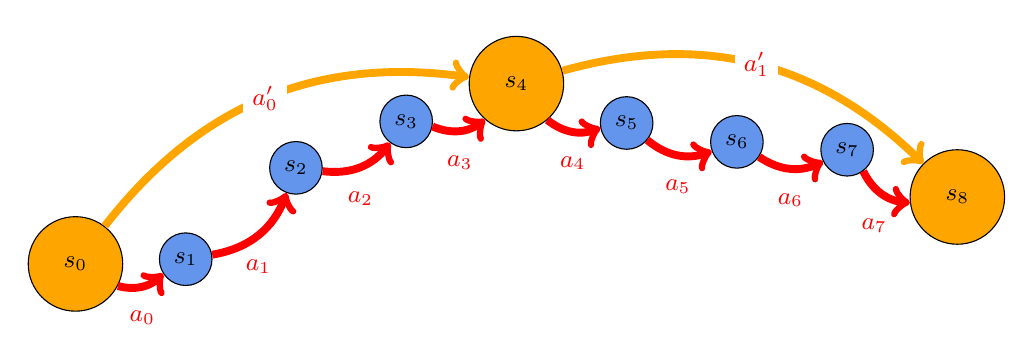
\begin{tikzpicture}
        % Define parameters
        \def\smallradius{0.3cm}
        \def\bigradius{0.6cm}
        \def\arrowsize{1mm}

        \node[draw, fill=Orange, circle, minimum size=2*\bigradius](s0) at (0.0, 0) {$s_{0}$};
        \node[draw, fill=CornflowerBlue, circle, minimum size=2*\smallradius](s1) at (1.4, 0.06) {$s_{1}$};
        \node[draw, fill=CornflowerBlue, circle, minimum size=2*\smallradius](s2) at (2.8, 1.22) {$s_{2}$};
        \node[draw, fill=CornflowerBlue, circle, minimum size=2*\smallradius](s3) at (4.2, 1.81) {$s_{3}$};
        \node[draw, fill=Orange, circle, minimum size=2*\bigradius](s4) at (5.6, 2.29) {$s_{4}$};
        \node[draw, fill=CornflowerBlue, circle, minimum size=2*\smallradius](s5) at (7.0, 1.79) {$s_{5}$};
        \node[draw, fill=CornflowerBlue, circle, minimum size=2*\smallradius](s6) at (8.4, 1.55) {$s_{6}$};
        \node[draw, fill=CornflowerBlue, circle, minimum size=2*\smallradius](s7) at (9.8, 1.45) {$s_{7}$};
        \node[draw, fill=Orange, circle, minimum size=2*\bigradius](s8) at (11.2, 0.85) {$s_{8}$};

        \draw[->] (s0) edge[red, line width=\arrowsize, bend right] node[midway, xshift=0.0cm, yshift=-0.4cm, color=red]{$a_0$} (s1);
        \draw[->] (s1) edge[red, line width=\arrowsize, bend right] node[midway, xshift=0.0cm, yshift=-0.4cm, color=red]{$a_1$} (s2);
        \draw[->] (s2) edge[red, line width=\arrowsize, bend right] node[midway, xshift=0.0cm, yshift=-0.4cm, color=red]{$a_2$} (s3);
        \draw[->] (s3) edge[red, line width=\arrowsize, bend right] node[midway, xshift=0.0cm, yshift=-0.4cm, color=red]{$a_3$} (s4);
        \draw[->] (s4) edge[red, line width=\arrowsize, bend right] node[midway, xshift=0.0cm, yshift=-0.4cm, color=red]{$a_4$} (s5);
        \draw[->] (s5) edge[red, line width=\arrowsize, bend right] node[midway, xshift=0.0cm, yshift=-0.4cm, color=red]{$a_5$} (s6);
        \draw[->] (s6) edge[red, line width=\arrowsize, bend right] node[midway, xshift=0.0cm, yshift=-0.4cm, color=red]{$a_6$} (s7);
        \draw[->] (s7) edge[red, line width=\arrowsize, bend right] node[midway, xshift=-0.1cm, yshift=-0.4cm, color=red]{$a_7$} (s8);

        \draw[->] (s0) edge[Orange, line width=\arrowsize, bend left] node[midway, color=red, fill=white]{$a'_0$} (s4);
        \draw[->] (s4) edge[Orange, line width=\arrowsize, bend left] node[midway, color=red, fill=white]{$a'_1$} (s8);

    \end{tikzpicture}
    \caption{Representation of the transitions made by a hierarchical agent. Orange actions and states represent global
    transitions. Light blue states and red actions represent local transitions.}
    \label{figure:bg:plan-rl:hierarchical-transitions}
\end{figure}

% CONTINUER à DEEPL WRITE ICI
% CONTINUER à DEEPL WRITE ICI
% CONTINUER à DEEPL WRITE ICI
% CONTINUER à DEEPL WRITE ICI
% CONTINUER à DEEPL WRITE ICI
% CONTINUER à DEEPL WRITE ICI
% CONTINUER à DEEPL WRITE ICI
% CONTINUER à DEEPL WRITE ICI
% CONTINUER à DEEPL WRITE ICI
% CONTINUER à DEEPL WRITE ICI
% CONTINUER à DEEPL WRITE ICI
% CONTINUER à DEEPL WRITE ICI

Figure~\ref{figure:bg:plan-rl:hierarchical-transitions} propose a representation of the global transitions compare to
the local ones.

We know why we might want to build this architecture, but the technical aspect of how to build a global policy stay a
mistery, let's demystify it.

\subsection{Various methods for hierarchical agents}\label{subsection:bg:plan-rl:global-actions}

Some methods may vary in the way they condition the control policy, or in the way they build and train the global
policy.

\textbf{Global actions} can take multiple types.
Our objective is to use it to select which task our local policy will perform.
The most trivial way to do so is to learn various policies, and select which one we want to do.
The most popular method is to learn \important{options}.
An option is defined by:
\begin{itemize}
    \item An initialisation condition $I_o(s)$ that define when the option can be started.
    \item A termination condition $\beta_o(s)$ that define when the option is done.
    \item A policy $\pi_o(s)$ that is the local policy selected for this option.
\end{itemize}
This paradigm has been introduced by \citet{sutton1999between}.

We can also have a single local policy, and condition it with the global action $a'$.
Then, the action $a'$ can be a goal, and $\pi_l$ is a goal-conditioned policy, a policy conditioned by a goal that
received higher rewards when the agent is considered close to the goal by a hand-design criteria.

These are the most used conditioning types in the literature, but we can imagine other global actions, such integers in
a bounded global action set $A'$, that will condition a single local policy that will learn as many macro-actions that
there is possible global actions.

\textbf{Global policy.} In hierarchical agent, the global policy can of course be trained with reinforcement learning.
In this context, the global policy action space $A$ could be the local policy goal space $G$ if the local policy is
goal-conditioned, or a discrete space for the other global actions types presented previously.
But the global policy is not necessarily trained with reinforcement learning.
It can also be any imaginable policy that produce one of the macro action types we presented earlier, such as a 
reachability graph.
This data structure is the same that the one we defined in Section~\ref{section:bg:planning},
Definition~\ref{definition:bg:plan:classical-planning-model}.
Solve the shortest path problem in this reachability graph then gives us a sequence of actions and nodes.
If the local policy is goal-conditioned, the nodes can be used as a sequence of sub-goals for the local policy, and can
then be used as global actions.
If the local policy is a sequence of policies or a single policy conditioned by discrete global actions, the actions
that composed the plan (the edges in the reachability graph), can be used as global actions.

We motivate the concept of hierarchical agent by claiming it could divide a tough problem into easier sub-problems.
Now we better understand how such architectures can be implemented, we can better understand which problems it answers
and how.

\subsection{Impact of hierarchical agents on RL problems}\label{subsection:bg:plan-rl:impact-on-rl-problems}

We presented a large but nonetheless non-exhaustive list of problems associated with RL in this chapter
(Section~\ref{subsection:bg:rl:challenges-in-reinforcement-learning}).
Some of them could be limited by the usage of a hierarchical agent architecture.

\textbf{Credit assignment.}\label{paragraphe:bg:plan-rl:impact:credit-assignment}
We introduced the idea that the global policy is interacting with a different transition function than the one induced
by the environment.
This global transition function $P'(s_{t+H} | s_t, a')$ leads the global actions to have a bigger temporal impact than
the local actions.
In other words, for a single global action $a'$, our global agent will perform $H$ steps in the environment.
From its perspective, the global agent will associate the reward, or the value of the new state $s_{t+H}$ to the global
action $a'$ and to the state $s_t$.
For the credit assignment problem (Subsection~\ref{subsection:bg:rl:challenges-in-reinforcement-learning}), it implies
that the value of a state is propagated $H$ time faster to the state-action pairs that could lead the agent to it.
If the global policy will have a research space of an equivalent size of a single policy RL agent, it will learn way
faster due to this sample-efficient credit assignment.

\textbf{Exploration.}

% NOTE: Je pourrais définir plus formellement ce que j'entend par diversité, ou ce que j'entend par la maximisation de
% la couverture de l'espace d'état, mais je ne les utiliserait pas donc pour le moment je laisse comme ça.

The term exploration is quite large.
Some will say that it is maximised when we select each action with a uniform probability.
Others will say that it is maximised when the coverage of the state space $S$ by the states sampled by the policy since
the beginning of the training is maximal.
It is important to make sure that a minimum of both kind of exploration is made by the agent, even if both will not
have the same importance depending on the problem we're trying to solve.
The first one makes sure that we don't let untested an action that might lead to high rewards.
The other one makes sure we find all possible high rewards which could help to find the actions leading to it.

The first definition is interesting in RL in general because we never know what will be the outcome of an action, so
they all have to be tested.
But it is quite easy in general to make sure we tested all actions from a state.
It is way harder to make sure we explored every possible states or maximise the state space coverage.

Global actions are interesting for exploration because they help to maximise the state-space coverage in some cases.
We explained in the Section~\ref{subsection:bg:rl:challenges-in-reinforcement-learning}, in the paragraphe about sparse
reward, that an agent trained with RL cannot navigate efficiently in the state space without finding rewards.
Because our local policy solve simpler tasks, with denser rewards, induced by the selected global actions, it will
navigate more efficiently in the directions of the sub-task, or global action, rewards.
Then, global actions will lead to a more efficient state space coverage because they will guide the agent in specific
directions in the state space, leading to an easier maximisation of its coverage.
But global actions needs a second characteristic to lead to a better state space coverage.
If all global actions $a' \in A'$ leads to the same local reward function for some reason, the local policy will be
guided in the same area of the state space for any global action, which doesn't really match the definition of space
coverage.
In general, hierarchical agents methods guarantee a minimum of diversity in the skills (the local policy conditioned
by a specific global action) produced by the agent.
This diversity makes sure that for a given global action, executed from a given state $s_t$, the states sampled by the
local policy will be different that the ones sampled by any other skills.

\textbf{Catastrophic forgetting and distribution shift}

In Section~\ref{subsection:bg:rl:challenges-in-reinforcement-learning}, we talked about the distribution shift problem.
In RL, this problem arise in many cases.
First of all, the exploration in the sens of state space coverage is never instantaneous, even without a hierarchical
agent.
Then, the policy will learn the best actions to perform in some states before to learn the best action to perform from
completely different states.
This implies that the policy will forget the best action to perform in the old states, unless it continue to learn them.
This implies that the bigger the state space is, the bigger the replay buffer (the memory of passed interactions) and
the training batch (the set of interactions to learn on at each training state) have to be, leading to computation
inefficiency in both space and time.
Use a hierarchical agent could help to solve this problem.
Learning options could be seen as a way to solve this distribution shift problem and the catastrophic forgetting induces
by it.
Indeed, each option only learn to be applied on a specific initial condition.
For other initial conditions (or in other words, other states) another policy will perform the subtask.
Then, each option will never forget the best actions to perform from these initial condition.
CURIOUS\citep{colas2019curious} algorithms is a hierarchical agent that learn various skills associated with human
designed reward functions.
The probability to select a skill to learn depends on the learning
progress\footnote{How much the agent is making progress at performing this skill while learning it.} of the agent on
this skill.
When a skill is forgot because others are learned, the agent will fail to do it but will rapidly learn back how to do
it.
The learning progress, and then the probability to learn a skill, increase when it is forgotten.
Hierarchical agents don't necessary help to solve this distribution shift problem, but they can allow to introduce
efficient mechanisms to solve it.
This architecture can also help to produce a local policy that is efficient for domain adaptation, but we will detail it
in Chapter\ref{chap:rgl}.

Understanding why the hierarchical agents architecture can solve these problems, and most of all keeping in mind which
problems it can solve, helps us to better understand when such architecture is useful.
